\documentclass[,]{sagej}

\usepackage{moreverb,url,natbib, multirow, tabularx}
\usepackage[colorlinks,bookmarksopen,bookmarksnumbered,citecolor=red,urlcolor=red]{hyperref}



\usepackage{hyperref}
\usepackage[utf8]{inputenc}
\usepackage{dcolumn}
\def\tightlist{}


\begin{document}

\title{WFH and broadband speed (title needs rework)}

\runninghead{}

\author{A. N. Author\affilnum{}, John Smith\affilnum{}}

\affiliation{}



\begin{abstract}
TBC
\end{abstract}

\keywords{covid; internet; working from home; broadband speed; time-series
clusters}

\maketitle

\hypertarget{sec:1}{%
\section{Introduction}\label{sec:1}}

During the pandemic, working from home using digital technologies,
whether partially or exclusively, was transformed from a niche means of
accessing work, albeit one that had been on a slow, upward trend, to a
widespread way of life in many countries. The ability to work from home
or telecommute meant millions retained their jobs and, to a varying
extent, maintained productivity during periods of strict lockdowns
around the world. However, this ability has not been evenly distributed
socially or spatially, creating a new type of digital divide. On one
side are those who can work from home, supported by digital
technologies, and have thus been able to enjoy both economic resilience
and greater personal safety. On the other side, previously employed
individuals have been forced to accept furlough or redundancy packages
unless they are part of the cadre of essential workers, who are
potentially at high risk of infection. Whilst the basis for this new
digital divide has been viewed as mainly occupational, here we consider
whether the divide is also technological.

Using the UK as a case study, this paper aims to understand how the
quality and reliability of internet service, as reflected in
\emph{experienced} internet speeds, may reinforce or redress the spatial
and social dimensions of the digital division exposed by the pandemic.
To do so, we employ volunteered geographic data on individual broadband
speed tests and state-of-the-art time-series clustering methods to
create clusters of UK local authorities with similar temporal signatures
of experienced internet speeds. We then associate these clusters of
local authorities with their socioeconomic and geographic
characteristics to explore how they overlap with or diverge from the
existing economic and digital geography of the UK. Our analysis enables
us to better understand how the spatial and social distribution of both
occupations and online accessibility intersect to enable or hinder the
practice of telecommuting at a time of extreme demand. We will also
consider what lessons can be learned from this time for a future where
telecommuting is likely to remain a more common means of accessing work,
at least in comparison to the pre-Covid era, and broadband services and
infrastructure must be fit for purpose. \textbf{LET'S LEAVE IT FOR NOW,
BUT I THINK WE CAN CRYSTALISE MORE THE RQ}

The capability to work from home has previously been studied from the
perspective of whether work tasks in a given occupation both can be and
are allowed to be performed using digital technologies independently of
location or co-location with colleagues, including supervisors
\citep{allen2015effective, singh2013modeling}. However, successful
telecommuting also requires that the quality and reliability of digital
services, particularly home internet connection speeds, enable the
completion of work tasks with a minimum of delay or interruption. Prior
to the pandemic, the performance of broadband services with respect to
telecommuters was never tested at scale, as working from home and
connecting to colleagues and workplace resources via the internet was
the purview of a small minority of workers. Instead, leisure use in the
evening, when video streaming services are at their peak, has been used
to benchmark broadband performance and service delivery by different
Internet Service Providers (ISPs), at least in the UK \citep{ofcom2017}.

Yet the shift towards telecommuting during various stages of lockdown
around the world has been drastic and there are speculations that
post-Covid, the tendency to work from home will be much higher than
pre-Covid, raising questions around whether internet services can
accommodate the increased demand. For example, \(47\)\% of people in
employment in the UK worked solely from home in April \(2020\), whilst
the same figure only reached \(5\)\% the year before
\citep{ons2020, ons2020lm2019}. A back of the envelope calculation
suggests that up to 40\% of the working force could work from home on an
ongoing basis \citep{batty2020editorial}. Similar figures have been
reported for other countries \citep{felstead2020homeworking}. For
instance, \(37\)\% of the European workforce worked from home in April
\(2020\) with countries like Finland reaching \(60\)\%
\citep{eurofound2020}. In the US, almost half of the working population
worked from home during the same period because of the pandemic
\citep{brynjolfsson2020covid}, and a recent estimate indicated that
\(37\)\% of all jobs in the US can be permanently performed entirely
from home \citep{NBERw26948}.

None of these changes could have happened in the absence of reliable
information and communication technology (ICT) infrastructure -- both in
terms of software and hardware. But while software innovations are
easily diffused across space and society\footnote{See for example the
  huge success of videoconferencing apps such as Zoom
  \citep{marks2020zoom}.}, the same does not apply for ICT hardware
infrastructure such as internet broadband connectivity. The literature
describes first level digital divides in terms of the availability and
quality of internet connectivity, such as that manifest in different
geographies in the UK
\citep{riddlesden2014broadband, philip2017digital}. Second level digital
divides consider the presence or lack of the necessary skills to
effectively utilise digital technologies and the internet
\citep{blank2014dimensions, van2011internet}. The third level focuses on
the heterogenous returns of internet usage among different socioeconomic
groups and, consequently, how digital technologies can assist in
bridging or further enhancing existing socioeconomic divides.
\citep{stern2009levels, van2014digital, van2015third}. The capability to
telecommute is related to all three levels of digital divides, but more
importantly leads to differentiated outcomes regarding the economic
resilience of people and places to overcome a systemic shock such as the
current pandemic. The extreme level of demand for telecommuting
fundamentally alters the potential returns of internet use for the user
and wider community, assumes skills or functions that are present in
some occupations but not in others, and relies upon access to high
quality internet services.

As the quality of internet infrastructure and services, as well as
variation in occupations are spatially dependent and clustered in space,
our approach offers a framework for understanding the impact of and
interactions between the different levels of digital division in
different places with different characteristics. By asking how resilient
broadband speeds, and particularly upload speeds are as experienced in
different parts of the UK during a time of extreme demand, we
interrogate which places benefit from the greater economic resilience
digital technologies can offer, not only during the pandemic, but also
into the future. The structure of this paper is as follows. First we
review the literature on telecommuting and digital divides to better
understand the structural and spatial development of these practices
pre-pandemic, and thus their importance to the economic resilience of
different places. We then describe our data and methodology. Our results
section first offers a classification of how internet services vary
across the UK local authorities and then assesses whether these clusters
replicate or repudiate other socio-economic and geographic patterns of
economic resilience. The paper ends with a conclusions section.

\hypertarget{sec:2}{%
\section{Literature review}\label{sec:2}}

\hypertarget{sec:2.1}{%
\subsection{From telecommuting to \#WFH}\label{sec:2.1}}

In this analysis, the terms `telecommuting' and `working from home' are
used interchangeably, as most remote labour during the Covid-19 crisis
was carried out in the homes of individual employees rather than any
other location \citep{eurofound2020}. However, it should be noted that
previous research has explored how telecommuting can occur in other
places, including satellite offices or on public transport
\citep{felstead2012rapid, siha2006telecommuting}. Previous research has
also used a variety of definitions to measure the level of telecommuting
within different workforces, distinguishing, for example, between those
directly employed, indirectly employed, self-employed, full-time or
part-time, and those who use digital technologies to work remotely
full-days or part-days
\citep{allen2015effective, bailey2002review, haddad2009examination}. No
matter the definition, the option and capability to telecommute or work
from home has never been equally distributed spatially or
socio-economically any more than different industries and employment
opportunities have. For example, studies from the United States, the
Netherlands, and the UK found that telecommuters are most likely to hold
professional, managerial, and technical occupations where the workforce
is better educated and wealthier, and that there is suppressed demand
among women and part-time workers
\citep{headicar2016move, peters2004employees, singh2013modeling}.

Opportunities for working from home during the current pandemic have
likewise not been equally spread across the workforce.
\citet{NBERw26948} indicated that in the US, managers, educators, as
well as those working in computer-related occupations, finance, and law
can easily work from home, and that occupations with opportunities to
telecommute are associated with higher earnings. This is not the case
for the workforce occupied in more spatially fixed occupations, from
farming, construction and manufacturing to hospitality and care
services. In the US, these occupations tend to be lower-income,
non-white, without a university degree, live in rental accommodation and
lack health insurance \citep{NBERw27085}. Similar trends can be observed
for other countries. For example, \(75\)\% of workers with tertiary
education worked from home in Europe during spring \(2020\), whilst only
\(34\)\% of workers with secondary education and \(14\)\% of those
primary education did so \citep{eurofound2020}.

\hypertarget{sec:2.2}{%
\subsection{Digital divides and economic resilience}\label{sec:2.2}}

Our understanding of telecommuting as a product of enabled occupations
can be described as a manifestation of the third level digital divide,
as those who are able to use digital technologies to work from home
benefit from a high rate of return on their use of the internet in terms
of autonomy, flexibility, and time saved from commuting
\citep{peters2004employees, siha2006telecommuting, singh2013modeling}.
These returns have been even greater during the Covid-19 crisis, when
those with the ability to telecommute also have the ability to maintain
their employment whilst protecting their health. However, the success of
these arrangements has been dependent upon the first level digital
divide, which is associated with access and quality of internet
connectivity at a time of extremely high demand. \citet{SALEMINK2017360}
provides a systematic review of the pre-pandemic, first level digital
divide in infrastructure quality between urban and rural areas in
various advanced economies. Rural areas, predictably, fare worse. Yet
whether this variation in infrastructure quality affects the spatial
footprint of telecommuting has not previously been measured, in part
because telecommuting has not previously been the cause of greatest
demand and pressure on internet services.

There are indications that those who purchase high speed connections
consume more data of all sorts and use their connections for a variety
of purposes \citep{hauge2011consumer}, and that there is a correlation
between access to internet services and a reduction in household
transport spend \citep{bris2017ict}. Whether the implication is more
internet use and less travel because of increased telecommuting, these
studies suggest that better internet services enable households to make
savings and efficiencies, an example of the first level digital divide
reinforcing the third level. Yet did the purchase of high speed
connections and increased internet access also prepare households for
long-term home-working, enforced by government restrictions? The extreme
demand during the pandemic provides a new opportunity to understand how
infrastructure accessibility, quality, and reliability affects
telecommuting, particularly in light of the high volumes of
bandwidth-intensive video conferencing required in order to avoid the
face-to-face contact that could increase the spread of infection. We
seek to answer how internet service resilience contributes to or reduces
economic resilience when the latter is dependent upon the capability to
work from home. We also aim to improve our understanding of the impact
of first level digital division on telecommuting, and whether this
results in much more fundamental third level digital division than has
previously been perceived.

Furthermore, these multi-layered digital divides intersect with material
divides and the economic geography of the UK. Following the regional
economic resilience literature, which underlines the differentiated
capacity of cities and regions to escape or recover from economic crises
\citep{martin2012regional, kitsos2018economic}, different places have
different industrial and occupational profiles, and these affect the
aggregated potential capacity of places for telecommuting. Such profiles
are associated with longstanding inequalities in the UK and their
spatial representation as a North-South divide
\citep{martin_north_south}. Various studies have illustrated severe
inequalities between the north and the south regions of England
\textbf{replace `UK'} regarding, for example, skills and human capital,
unemployment, productivity and prosperity
\citep{lee2014grim, mccann2020perceptions, dorling2018peak}. Some
scholars have even argued that the UK suffers some of the highest level
of interregional inequalities in the global north
\citep{gal2018reducing, mccann2016uk}. Not only are all three levels of
digital divides associated, to a certain extent, with or shaped by the
geography of the UK, but the intersection of the digital and material
divides affects the capacity of places to overcome some of the economic
effects of the Covid-19 pandemic. Importantly, this is the first time
that digital technologies became an essential tool for economic
resilience for such a great part of the population.

\hypertarget{sec:3}{%
\section{Methods and data}\label{sec:3}}

\hypertarget{sec:3.1}{%
\subsection{Time-Series Clustering}\label{sec:3.1}}

The starting point of our methodological framework is cluster analysis,
which can be defined within the modern machine learning framework as an
unsupervised learning task, partitioning unlabelled observations into
homogeneous groups known as clusters \citep{montero2014tsclust}. The key
idea is that observations within clusters tend to be more similar than
observations between clusters. Clustering is particularly useful for
exploratory studies as it identifies structures within the data
\citep{aghabozorgi2015time}. Therefore, cluster analysis is a widely
used family of techniques in geography
\citep{gordon1977classification, everitt1974cluster}. For instance,
clustering methods are the basis of \emph{geodemographics}, a research
domain which aims to create small area indicators or typologies of
neighbourhoods based on various and sometimes diverse variables
\citep{SINGLETON2009289, harris2005geodemographics}. Clustering
techniques have also been employed to solve \emph{regionalisation}
problems \citep{niesterowicz2016}.

Common characteristics of these studies are the cross-sectional nature
of the data they employ. Indeed, most clustering problems in geography
deal with observations that are fixed in time. However, for this paper
we are interested in internet speeds, which vary over time and,
therefore, create clusters of local authorities in the UK with similar
temporal signatures of experienced internet speeds. Hence, we deviate
from the established geographical clustering tools and employ
time-series clustering methods.

Time-series clustering methods have been developed in order to deal with
clustering problems linked to, for instance, stock or other financial
data, economic, governmental or medical data as well as machine
monitoring
\citep{aggarwal2013time, aggarwal2001surprising, hyndman2015large, WARRENLIAO20051857}.
The main challenge -- and also the difference with cross-sectional
clustering problems -- is data dimensionality given the multiplicity of
data points for every individual object, local authorities in our case,
included in the data set. Time-series are dynamic data as the value of
the observations change as a function of time
\citep{aghabozorgi2015time}. This high dimensionality leads to (i)
computational and algorithmic challenges regarding handling these data
and building algorithms to perform clustering over long time-series, and
(ii) open questions regarding the choice of similarity measures in order
to cluster similar times series objects together considering the whole
length of the time-series and overcoming issues around noise, outliers
and shifts \citep{lin2004iterative, aghabozorgi2015time}.

For this paper we utilise a category of time-series clustering methods
known as shape-based approaches. These methods match two sperate
time-series objects based on the similarity of their shapes through the
calculation of distances between the shapes, and are thus better
equipped to capture similarities between short length time-series
\citep{aghabozorgi2015time}. This approach serves best this paper
because (i) we identify clusters of UK local authorities with similar
temporal signatures -- i.e.~shapes -- of experienced internet speeds and
(ii) the length of our time-series is short (see the data discussion in
this section).

Another import element of time-series clustering is the actual
clustering algorithm. Similar to the clustering of cross-sectional data,
we can employ partitioning algorithms, which lead to non-overlapping
clusters, hierarchical clustering, which classifies clusters at
different levels, and fuzzy algorithms, which create overlapping
clusters \citep{sardatime}. Because of the simplicity of the
implementation and the interpretability of the results, we utilise here
partitioning clustering based on the widely used \emph{k}-means
algorithm. This is an iterative algorithm, which begins with defining
the desired number of clusters \emph{k}. Then each observation is
randomly assigned to a cluster from the \([1,k]\) space. This initial
cluster assignment is followed by iterations in order to minimise the
distance between the centroids of the clusters and the observations
assigned to these clusters \citep{james2013introduction}.

There are a number of differences between the above described
application of \emph{k}-means for cross-sectional data and its
application for times series data. Instead of creating clusters around
centroids, a common approach is to create clusters around
\emph{medoids}, which are representative time-series objects with a
minimal distance to all other cluster objects \citep{sardatime}. Also,
instead of calculating the Euclidean distance between centroids and data
points, more complex distance measures need to be employed in order to
capture the similarity between a time-series object and a medoid. A
common distance measure for shape-based time-series clustering is
Dynamic Time Warping (DTW). Using its underpinning dynamic programming
algorithm, DTW compares two time-series objects to find the optimum
warping path between them. DTW is widely used in order to overcome
limitations linked to the use of Euclidean distance
\citep{sardatime, berndt1994using, ratanamahatana2004everything}. The
\texttt{R} package \texttt{dtwclust} has been used for the time-series
clustering \citep{dtwclust}.

\hypertarget{sec:3.2}{%
\subsection{Experienced Broadband Speeds}\label{sec:3.2}}

To assess the quality and reliability of internet across local
authorities in the UK during the time when the population were told to
work from home if at all possible we utilise unique data comprising
individual internet speed tests from Speedchecker Ltd\footnote{\url{https://www.broadbandspeedchecker.co.uk/}}.
This is a private company that allows internet users to check their own
broadband upload and download speeds, and stores every speed-check with
timestamp and geolocation information. These data have been used before
to assess digital divides \citep{riddlesden2014broadband} and the impact
of local loop unbundling regulatory processes
\citep{nardotto2015unbundling}. By using volunteered geographic data, we
are able to assess the \emph{experienced} internet speed by users, which
may differ from the \emph{advertised} maximum speeds of ISPs.

We are particularly interested in upload speeds and the frequency of
speed tests over the period from March to May \(2020\), as government
statements indicate this is when UK workers were told to work from home
if at all possible \citep{GovUK2020}. Average upload speeds are slower
than average download speeds, at \(9.3\)Mb/s mean upload speed for the
whole sample during the period of interest, compared to \(29.6\)Mb/s for
download speeds, but they are also less associated with internet-based,
high-demand, leisure activities such as video streaming. Therefore,
upload speeds are more relevant to work-related activities such as
uploading documents or two-way audio, video, and text-based
communication systems. Meanwhile, the frequency of speed tests was
important in identifying the temporal profile which would give us most
insight into experienced internet service and resilience, and provide an
indication of the volume of experience over particular units of time.

The first step in the workflow after dropping some outliers following
\citet{riddlesden2014broadband} was to transform the individual,
geolocated and time-stamped tests to more meaningful aggregates both in
terms of space and time. The frequency of testing indicates that whilst
there is an overall trend of increased testing from March to April and
then a slight reduction from April to May, this trend masks substantial
variation by not only the day of the week, but also time of day, as can
be seen in Figure \ref{test2020}. Thus, a daily aggregation of upload
speeds would mask the variation in experienced service over the course
of each weekday. Furthermore, the importance of this variation is
highlighted by a comparison with the same period in \(2019\), as in
Figure \ref{test2019}, when the volume of testing and thus of experience
of internet service quality was much more tied to the evening leisure
peak and presumably to download speeds. Since the increase in testing
during the working day in \(2020\) is an indication that users have a
greater perception of the variable quality of internet service,
particularly during a new morning peak of testing for service
reliability, we decided to include a measure of hourly variation in our
temporal profiles.

However, although this is a large data set -- \(241,088\) individual
tests performed during weekday hours across the study period -- there
are not enough observations for each Local Authority District (LAD) and
for each working hour of each working day -- \(631\) speed tests per LAD
on average -- to profile speeds at that level of detail. Therefore, we
aggregate all the speed-checks during the \(13\) weeks of March to May
inclusive for weekdays in \(2020\) by each hour of the day and day of
the week. As our research aims to identify the geography of internet
service resilience for work purposes, bank holidays and the hours
between midnight and \(6:00\) were excluded, as well as weekend days.
The composite week time-series thus comprise \(18\) hours multiplied by
\(5\) weekdays or \(90\) time points per series. We also aggregate these
data spatially because we could not follow individuals or households and
connect data points. The time-series were calculated for each of the
\(382\) LADs in the UK, standardised, and then a \emph{k}-means
partitioning around medoids clustering algorithm was applied using DTW.
We initially run the algorithm for \(k \in \mathbb{N} \bigcap [5,15]\)
and used cluster validity indices (CVIs) to pick the optimal solution of
\(k = 13\). Following \citet{sardatime} the majority vote for the
following CVIs was used: Silhouette (max), Score function (max),
Calinski-Harabasz (max), Davies-Bouldin (min), Modified Davies-Bouldin
(DB*, min), Dunn (max), COP (min).

\begin{figure}
\centering
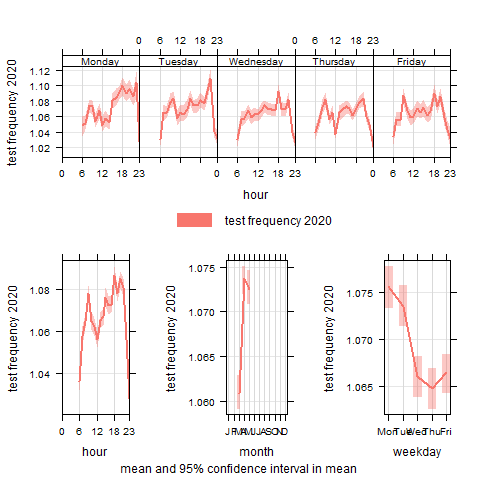
\includegraphics[width=0.75\textwidth,height=0.4\textheight]{figures/time.var.plot2020.png}
\caption{Speed tests over time, 2020 \label{test2020}}
\end{figure}

\begin{figure}
\centering
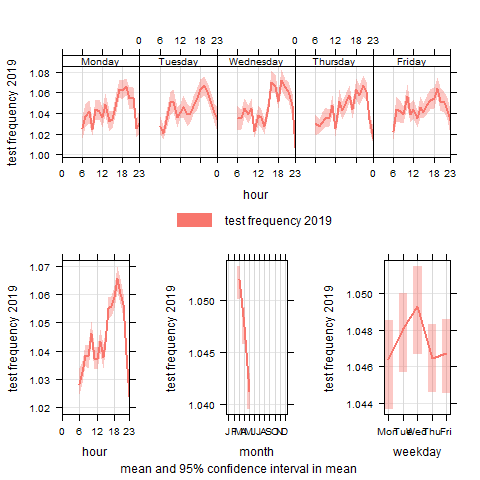
\includegraphics[width=0.75\textwidth,height=0.4\textheight]{figures/time.var.plot2019.png}
\caption{Speed tests over time, 2019 \label{test2019}}
\end{figure}

In Section \protect\hyperlink{sec:4.1}{4.1}, we review the temporal
profile of upload speed by hour of the day and day of the composite
week, as well as the experienced speed characteristics of each cluster.
Since the quality and reliability of internet services vary in time and
space due to both supply and demand-side influences, we use a number of
different measures to describe experienced upload speeds per cluster.
These include: a) mean, experienced connection speed, b) standard
deviation or the amount of fluctuation from the mean, and c) the
variation in speeds at particular times of day when working from home is
more likely to take place. We take account of all three measurements in
our descriptive statistics of upload speeds in order to determine how
resilient broadband speeds are as experienced in different parts of the
UK during a time of extreme demand.

The cause of these different experiences of broadband resilience may be
different in different areas, as they may reflect either similarities in
patterns of demand or similar quality of infrastructure. Our approach is
also limited by potential endogeneity, as for example, better quality
connections with high mean speeds may enable more working from home, but
greater demand may cause slower speeds, less reliability and greater
variability of speed at different times of day or week. Therefore, we
avoid attributing any cause to our analysis of the experienced level of
quality and reliability of upload speeds. Instead, we run an auxiliary
regression in order to understand how the spatial and temporal patterns
of internet service relate to the economic geography of the UK. More
specifically, we estimate the following multinomial model:

\begin{align}
Pr(Y_{i}=j) = \frac{exp^{X_{i}\beta_{j}}}{\sum_{i=1}^j exp^{X_{i}\beta_{j}}}
\begin{cases}
    i = 1, 2, ... , N \\  
    j = 1, 2, ... , J
\end{cases}\label{eq1}
\end{align}

Based on the outcomes of the time-series clustering, we identify \(J\)
distinct and crisp clusters. We then regress this cluster membership
against a vector \(X_{i}\) of socio-economic and geographic variables,
which are discussed in detail in the relevant Section
{[}4.2{]}{]}(\#sec:4.2), in order to explore how the different patterns
might support or undermine efforts to work from home and maintain safe
productivity and whether they reinforce existing spatial and social
inequalities. This analysis enables us to provide a more nuanced
understanding of how telecommuting and technology intersect at a time of
extreme demand, and what lessons this time has for a future where
telecommuting is likely to remain a common means of accessing work and
broadband services, as well as infrastructure, must be fit for purpose.

\hypertarget{sec:4}{%
\section{Results}\label{sec:4}}

\hypertarget{sec:4.1}{%
\subsection{Upload Clusters / cluster description}\label{sec:4.1}}

The temporal profiles of the local authority clusters have been
summarised in Figures \ref{UpClusterL} and \ref{UpClusterS} and Table
\ref{up.cluster.descr}. The graphs show a composite profile of mean
upload speeds per hour per day for each cluster, with the largest, in
terms of the LAD membership and population, five clusters in Figure
\ref{UpClusterL}, and the next six in Figure \ref{UpClusterS}. These
figures and table provide a comprehensive overview of the quality and
reliability of experienced broadband in different parts of the UK, the
temporal clusters offering a novel approach to understanding spatial
disparity.

\begin{figure}
\includegraphics[width=0.95\linewidth]{figures/upClusterL} \caption{\label{UpClusterL}Temporal profilies for upload speed large clusters}\label{fig:unnamed-chunk-2}
\end{figure}

\begin{figure}
\includegraphics[width=0.95\linewidth]{figures/upClusterS} \caption{\label{UpClusterS}Temporal profilies for upload speed small clusters}\label{fig:unnamed-chunk-3}
\end{figure}

\begin{table}[!htbp] \centering 
  \caption{Upload speed cluster characteristics\label{up.cluster.descr}} 
  \label{} 
\footnotesize 
\begin{tabular}{@{\extracolsep{0pt}} ccccccc} 
\\[-1.8ex]\hline 
\hline \\[-1.8ex] 
Cluster & N. of LADs & LAD population & mean speed & SD speed & mean AM speed & mean PM speed \\ 
\hline \\[-1.8ex] 
1 & 5 & 343100 & 8557 & 6139 & 7747 & 9563 \\ 
2 & 2 & 265600 & 10922 & 6687 & 9674 & 10645 \\ 
3 & 4 & 474700 & 10201 & 5658 & 9470 & 11236 \\ 
4 & 1 & 91100 & 9689 & 6122 & 7816 & 9689 \\ 
5 & 1 & 79800 & 10127 & 6024 & 9030 & 11101 \\ 
6 & 155 & 29535700 & 9397 & 5839 & 9161 & 9580 \\ 
7 & 4 & 559800 & 10119 & 6102 & 9813 & 11070 \\ 
8 & 5 & 436300 & 9429 & 6254 & 8682 & 10434 \\ 
9 & 32 & 6355500 & 10878 & 5957 & 10832 & 11071 \\ 
10 & 4 & 699600 & 10795 & 6005 & 9258 & 10697 \\ 
11 & 33 & 5771400 & 10845 & 5936 & 10781 & 10988 \\ 
12 & 10 & 1544900 & 9551 & 6166 & 9254 & 9048 \\ 
13 & 126 & 20277700 & 8392 & 5849 & 8299 & 8522 \\ 
\hline \\[-1.8ex] 
\multicolumn{7}{l}{Note: All speed measures are upload speeds} \\ 
\end{tabular} 
\end{table}

The second largest cluster, comprising \(126\) local authorities and
over \(20\) million people, is cluster \(13\). Cluster \(13\) has the
slowest aggregate mean upload speed of any of the clusters, and the
second highest ratio of the standard deviation to the mean. This
suggests that those living in local authorities in this cluster
experienced some of the lowest quality broadband services in terms of
upload speeds in the UK. However, the variation in upload speeds in
cluster \(13\), which can be an indication of its reliability, does not
seem to disproportionately affect the morning peak from
\(9:00\)-\(10:59\), as upload speeds are, on average, only \(2.6\)\%
slower than in the evening peak period between \(19:00\) and \(20:59\),
when entertainment purposes are likely to be using the most bandwidth.
In comparison, the five LADs that are home to \(343\) thousand people in
cluster \(1\) not only experience the second slowest mean upload speeds
and the highest ratio of standard deviation to the mean, but are also
much more affected during the morning peak.

Meanwhile, those living in the largest cluster -- \(6\), with \(155\)
LADs home to \(29.5\) million people, experience aggregate mean upload
speeds of about \(1\)Mb/s faster than those in cluster \(13\), but still
lower than the other three large clusters and most of the smaller
clusters, suggesting a middling quality of service. However, the time
profile for cluster \(6\) in Figure \ref{UpClusterL} shows that upload
speeds drop quickly from \(6:00\) to \(7:00\) on a Monday and peak
between \(23:00\) and midnight on Wednesday and Thursday, but tend to be
lower during the working day. Indeed, experienced mean upload speeds in
the morning peak are \(4.4\)\% lower than in the evening peak -- a
greater, more noticeable change than any of the other large clusters
experience, but smaller than any of the clusters with temporal profiles
shown in Figure \ref{UpClusterS}. Clusters \(8\) and \(12\) also have
mean upload speeds under \(10\)Mb/s, but higher than clusters \(1\) and
\(13\), and their standard deviation is not dissimilar. However, this
masks great variation in when lower speeds are experienced, with the
mean upload speeds much lower between \(9:00-10:59\) than between
\(19:00-20:59\) in cluster \(8\), but slightly faster in the morning in
cluster \(12\).

\begin{figure}
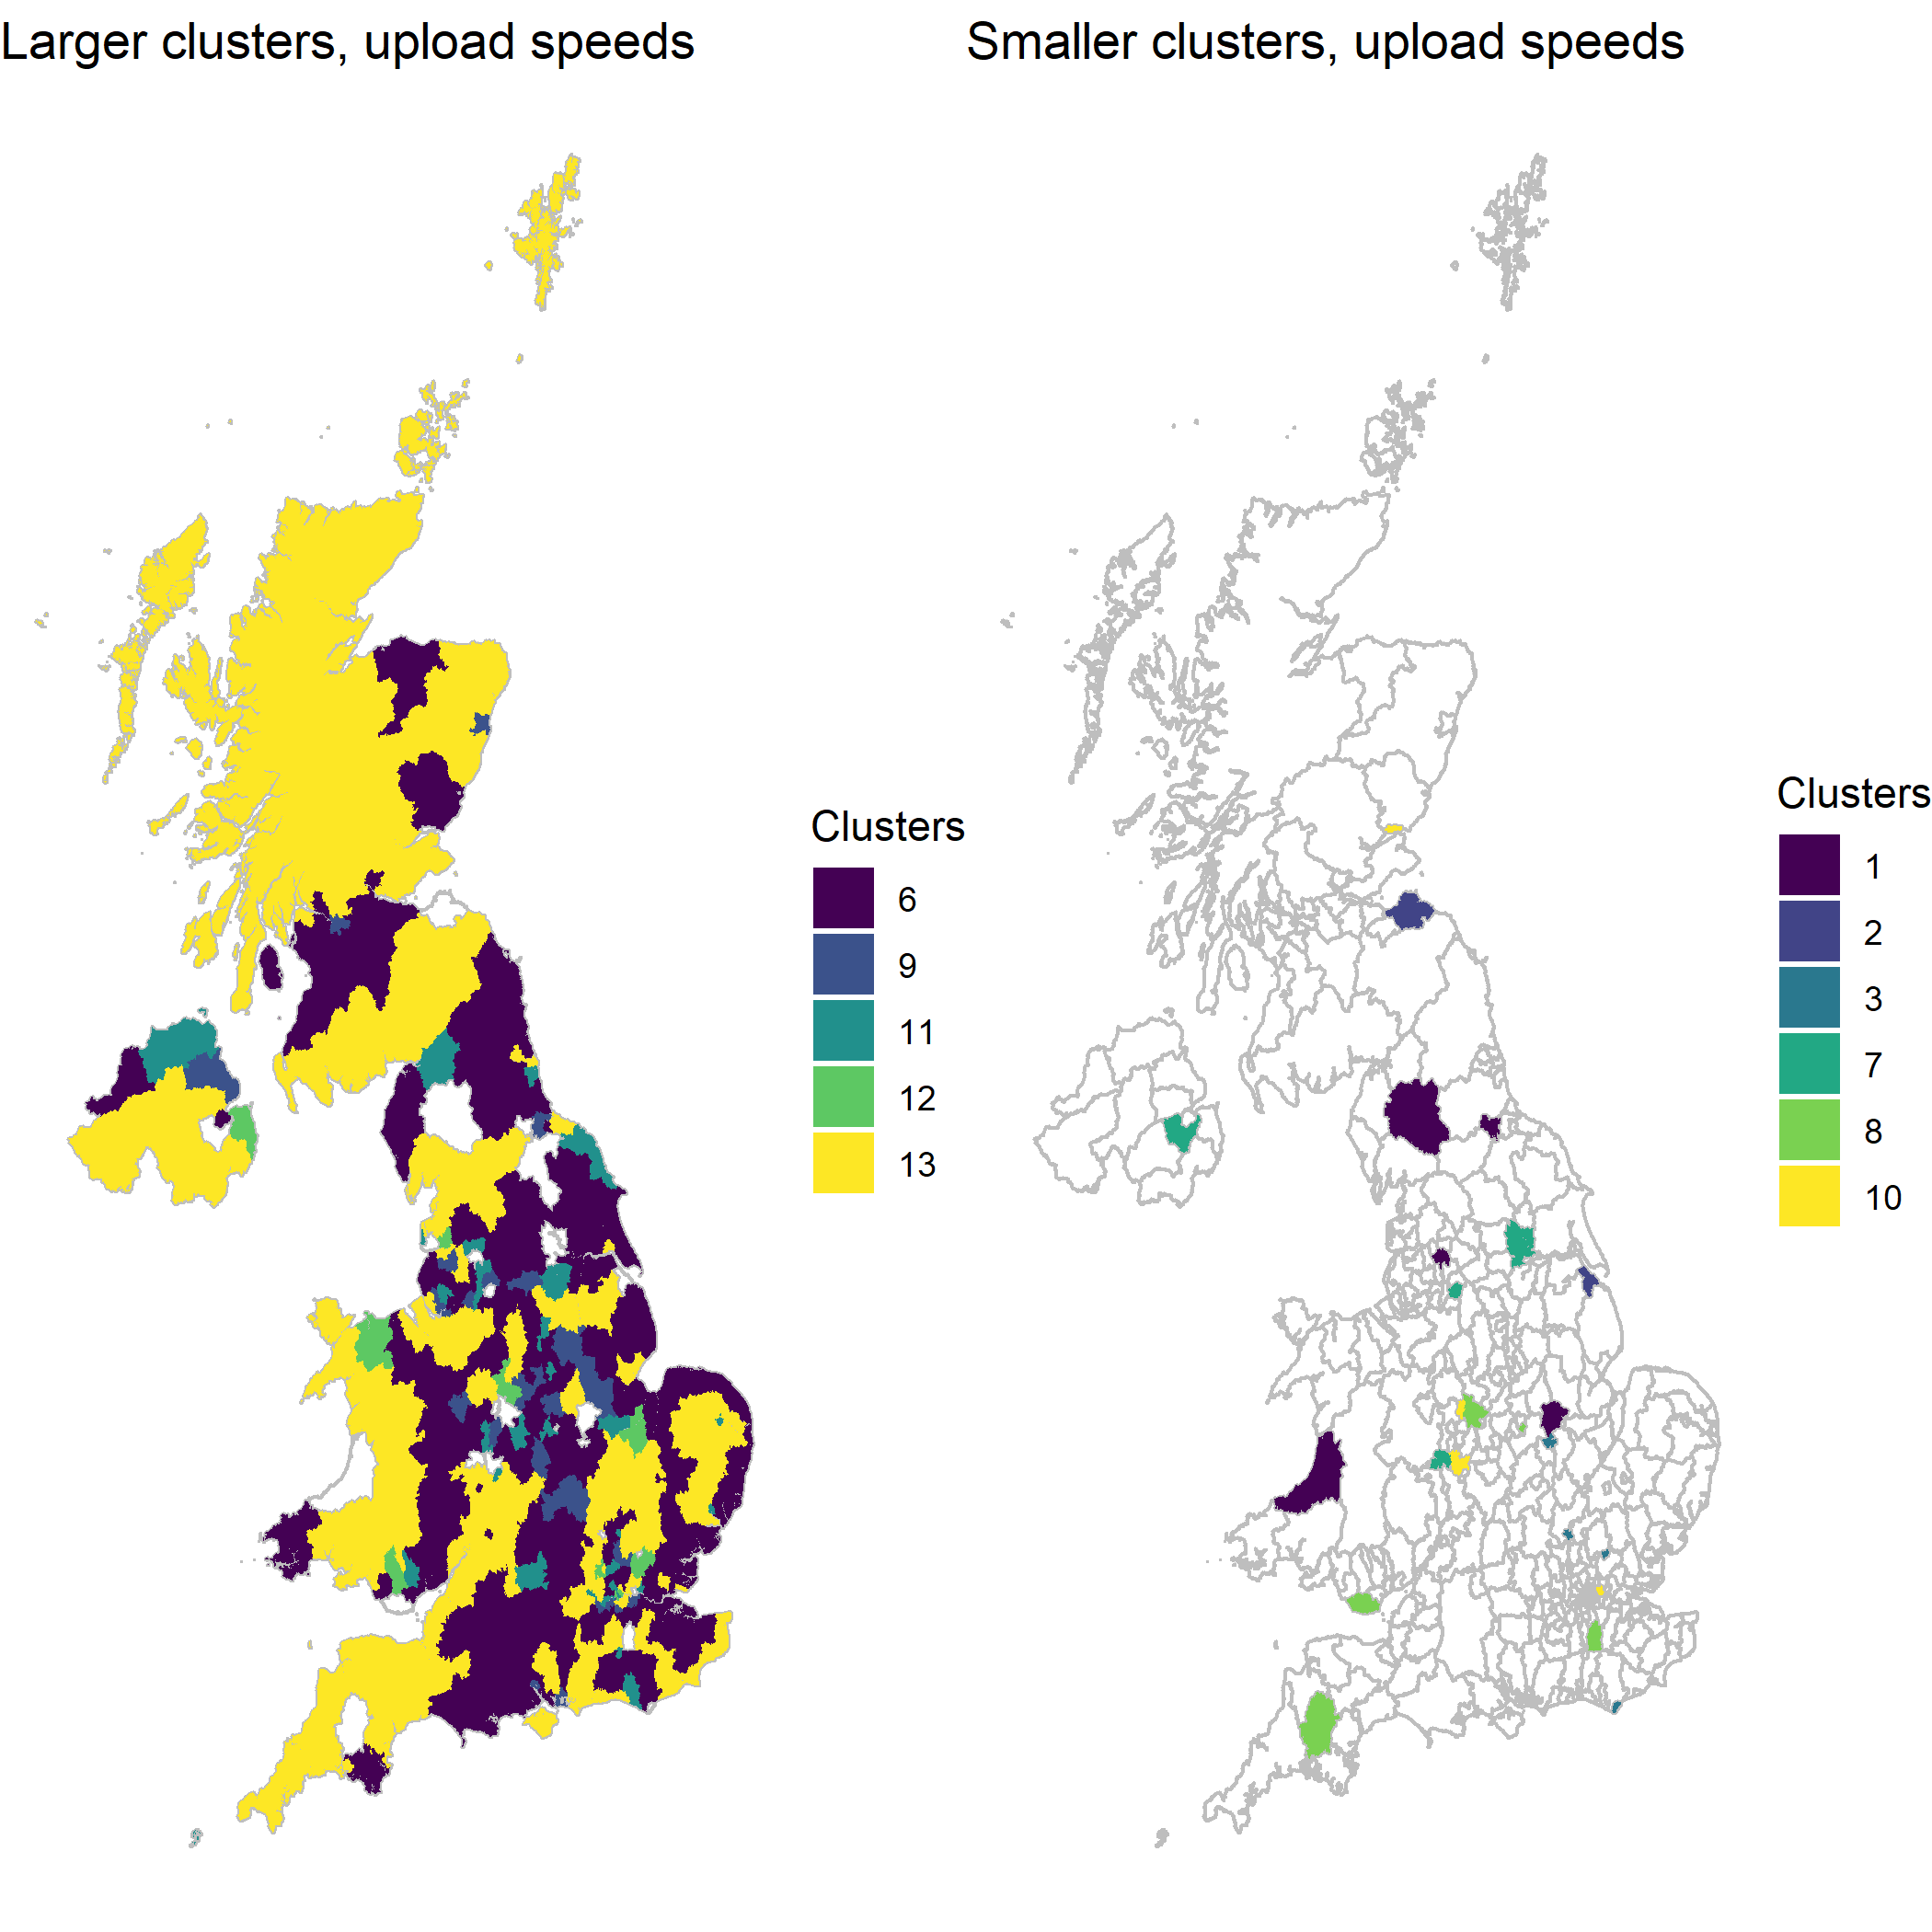
\includegraphics[width=0.95\linewidth]{figures/map.up.clusters} \caption{\label{map.up.clusters}Upload speed clusters for LADs}\label{fig:unnamed-chunk-5}
\end{figure}

Indeed cluster \(12\) is the only cluster to experience higher speeds in
the evening peak, compared to the morning peak, suggesting that
widespread telecommuting has generally changed the temporal profile of
internet activity throughout the UK. Yet even if all but one cluster is
showing slower speeds in the morning than the evening, the reliability
of internet services in different clusters during the working day still
varies considerably. Interpreting this variation from the large spikes
and dips shown on Figures \ref{UpClusterL} and \ref{UpClusterS} is
difficult, but the statistics in Table \ref{up.cluster.descr} show that
clusters \(9\) and \(11\) have the most reliable internet services. The
ratio of standard deviation to mean in both these clusters is below
55\%, and the ratio of upload speeds in the peak periods indicates that
speeds are only about 2\% slower in the morning. Mean speeds are also
higher than in any other cluster, excluding cluster \(2\), where
measures of reliability suggests poorer performance.

Thus, broadband services in clusters \(9\) and \(11\), home to over
twelve million people performed the best during the study period, in
terms of both quality and reliability. In Figure \ref{UpClusterL},
cluster \(11\) shows more noticeable peaks and troughs, but the lowest
points are not at the peak times described in Table
\ref{up.cluster.descr}. Rather, the slowest upload speeds on average
occur between \(6:00-7:00\) on Monday morning, \(14:00-15:00\) on
Friday, and \(16:00-17:00\) on Thursday. These slowest times are still
mostly faster than the average hourly upload speeds in cluster \(13\).
Finally, ignoring the smallest clusters in terms of population, that is
clusters \(4\) and \(5\), clusters \(3\), \(7\) and \(10\) also have
relatively high mean upload speeds. Clusters \(3\) and \(10\) pair high
mean speeds with low standard deviations relative to the mean speeds,
suggesting reliability and resilience, as well as quality broadband
services. Cluster \(7\) has a higher ratio of standard deviation to
mean, but there is less difference in average speeds between the morning
and evening peaks than in clusters \(3\) and \(10\).

In summary, the local authorities in clusters \(9\) and \(11\)
experienced resilient broadband internet that could support high levels
of telecommuting. Those in clusters \(2\), \(3\), \(7\), and \(10\) also
experience higher than average mean speeds and rank high to middle on
measures of service reliability. These LADs are \emph{not} on the wrong
side of the first level digital divide, but how likely are they to be
able to take advantage of their resilient ICT infrastructure and
services? Meanwhile, cluster \(6\) is not only the largest in terms of
number of LADs and population, it has the closest mean upload speed to
the pre-clustered average for the whole sample. As well as average
quality internet services, those in cluster \(6\) also experience
average reliability for work purposes, ranking fifth behind the four
other clusters with populations over one million, but ahead of the
smaller clusters. Clusters \(8\) and \(12\) are also close to average
mean upload speeds, but show very different patterns in terms of
reliability, whilst clusters \(1\) and \(13\) appear to suffer most from
a lack of quality internet services, with slow speeds and high standard
deviations. With those in cluster \(1\) in particular more likely to
experience that poor reliability during the morning peak, is this first
level digital divide occurring in areas where few are occupationally
able to telecommute anyway, and what are the implications for economic
resilience?

\hypertarget{sec:4.2}{%
\subsection{Post-clustering regression analysis}\label{sec:4.2}}

\begin{sidewaystable}[!htbp] \centering 
  \caption{Auxiliary multinomial regression of upload speed clusters on socio-economic and geographic LAD variables\label{aux}} 
  \label{} 
\tiny 
\begin{tabular}{@{\extracolsep{5pt}}lccccccccccc} 
\\[-1.8ex]\hline 
\hline \\[-1.8ex] 
\\[-1.8ex] & 1 & 2 & 3 & 6 & 7 & 8 & 9 & 10 & 11 & 12 & 13 \\ 
\\[-1.8ex] & (1) & (2) & (3) & (4) & (5) & (6) & (7) & (8) & (9) & (10) & (11)\\ 
\hline \\[-1.8ex] 
 pop, 2018 & $-$0.00004$^{***}$ & 0.00002$^{*}$ & 0.00001 & 0.00002$^{***}$ & 0.00002$^{***}$ & 0.00000 & 0.00002$^{***}$ & 0.00002$^{***}$ & 0.00002$^{***}$ & 0.00002$^{**}$ & 0.00002$^{***}$ \\ 
  & (0.00002) & (0.00001) & (0.00001) & (0.00001) & (0.00001) & (0.00002) & (0.00001) & (0.00001) & (0.00001) & (0.00001) & (0.00001) \\ 
  & & & & & & & & & & & \\ 
 job density, 2018 & $-$0.536$^{***}$ & $-$1.834$^{***}$ & $-$0.132$^{***}$ & $-$0.925$^{***}$ & $-$1.208$^{***}$ & $-$0.299$^{***}$ & $-$1.746$^{***}$ & $-$1.436$^{***}$ & 3.350$^{***}$ & 3.400$^{***}$ & 0.630$^{***}$ \\ 
  & (0.00000) & (0.00000) & (0.00000) & (0.00000) & (0.00000) & (0.00000) & (0.00000) & (0.00000) & (0.00000) & (0.00000) & (0.00000) \\ 
  & & & & & & & & & & & \\ 
 distance to nearest met. area & $-$0.034$^{***}$ & $-$0.014$^{***}$ & 0.002$^{***}$ & $-$0.020$^{***}$ & $-$0.074$^{***}$ & $-$0.044$^{***}$ & $-$0.013$^{***}$ & $-$0.036$^{***}$ & $-$0.031$^{***}$ & $-$0.036$^{***}$ & $-$0.024$^{***}$ \\ 
  & (0.0005) & (0.001) & (0.0002) & (0.002) & (0.0001) & (0.0002) & (0.002) & (0.0005) & (0.0003) & (0.0002) & (0.002) \\ 
  & & & & & & & & & & & \\ 
 distance to London & 0.007$^{***}$ & 0.002 & $-$0.016$^{***}$ & 0.001 & 0.004$^{***}$ & 0.004$^{***}$ & $-$0.002$^{*}$ & 0.005$^{**}$ & $-$0.002 & 0.003 & 0.006$^{***}$ \\ 
  & (0.001) & (0.002) & (0.0004) & (0.001) & (0.001) & (0.001) & (0.001) & (0.002) & (0.002) & (0.002) & (0.001) \\ 
  & & & & & & & & & & & \\ 
 South of the UK & $-$0.410$^{***}$ & $-$1.451$^{***}$ & $-$0.039$^{***}$ & $-$0.111$^{***}$ & $-$0.048$^{***}$ & $-$0.841$^{***}$ & $-$0.798$^{***}$ & 1.492$^{***}$ & 0.610$^{***}$ & 0.798$^{***}$ & 2.403$^{***}$ \\ 
  & (0.00000) & (0.00000) & (0.00000) & (0.00001) & (0.00000) & (0.00000) & (0.00001) & (0.00000) & (0.00001) & (0.00001) & (0.00001) \\ 
  & & & & & & & & & & & \\ 
 managerial jobs, 2020 & 0.939$^{***}$ & 0.704$^{***}$ & 0.435$^{***}$ & 0.704$^{***}$ & 0.316$^{***}$ & 0.786$^{***}$ & 0.576$^{***}$ & 0.311$^{***}$ & 0.476$^{***}$ & 0.594$^{***}$ & 0.615$^{***}$ \\ 
  & (0.00004) & (0.0001) & (0.00004) & (0.00004) & (0.00002) & (0.0001) & (0.00003) & (0.00003) & (0.00002) & (0.00004) & (0.00003) \\ 
  & & & & & & & & & & & \\ 
 tech jobs, 2020 & 0.096$^{***}$ & $-$0.257$^{***}$ & $-$0.071$^{***}$ & $-$0.111$^{***}$ & $-$0.206$^{***}$ & 0.199$^{***}$ & $-$0.126$^{***}$ & $-$0.606$^{***}$ & $-$0.180$^{***}$ & $-$0.398$^{***}$ & $-$0.112$^{***}$ \\ 
  & (0.00004) & (0.00004) & (0.00004) & (0.00003) & (0.00003) & (0.0001) & (0.00003) & (0.00003) & (0.00002) & (0.00004) & (0.00003) \\ 
  & & & & & & & & & & & \\ 
 skilled trade jobs, 2020 & 0.651$^{***}$ & 0.160$^{***}$ & $-$0.191$^{***}$ & 0.236$^{***}$ & 0.604$^{***}$ & $-$0.184$^{***}$ & 0.205$^{***}$ & 0.597$^{***}$ & 0.108$^{***}$ & $-$0.022$^{***}$ & 0.295$^{***}$ \\ 
  & (0.00004) & (0.00004) & (0.00003) & (0.00003) & (0.00003) & (0.00004) & (0.00002) & (0.00003) & (0.00003) & (0.00004) & (0.00003) \\ 
  & & & & & & & & & & & \\ 
 professional jobs, 2020 & $-$0.118$^{***}$ & $-$0.234$^{***}$ & $-$0.121$^{***}$ & $-$0.172$^{***}$ & $-$0.514$^{***}$ & $-$0.172$^{***}$ & $-$0.349$^{***}$ & $-$0.351$^{***}$ & $-$0.245$^{***}$ & $-$0.344$^{***}$ & $-$0.229$^{***}$ \\ 
  & (0.00005) & (0.0001) & (0.0001) & (0.00005) & (0.00003) & (0.0001) & (0.00004) & (0.0001) & (0.00003) & (0.00005) & (0.0001) \\ 
  & & & & & & & & & & & \\ 
 administrative jobs, 2020 & 0.019$^{***}$ & $-$0.836$^{***}$ & $-$0.040$^{***}$ & $-$0.117$^{***}$ & $-$0.139$^{***}$ & 0.206$^{***}$ & $-$0.058$^{***}$ & $-$0.200$^{***}$ & $-$0.055$^{***}$ & $-$0.168$^{***}$ & $-$0.177$^{***}$ \\ 
  & (0.00003) & (0.00002) & (0.00004) & (0.00001) & (0.00003) & (0.00003) & (0.00001) & (0.00002) & (0.00002) & (0.00002) & (0.00002) \\ 
  & & & & & & & & & & & \\ 
 leisure jobs, 2020 & $-$0.198$^{***}$ & $-$0.180$^{***}$ & $-$0.225$^{***}$ & $-$0.476$^{***}$ & $-$0.654$^{***}$ & $-$0.820$^{***}$ & $-$0.537$^{***}$ & $-$0.935$^{***}$ & $-$0.353$^{***}$ & $-$0.625$^{***}$ & $-$0.491$^{***}$ \\ 
  & (0.00002) & (0.00004) & (0.00004) & (0.00002) & (0.00002) & (0.00003) & (0.00002) & (0.00001) & (0.00002) & (0.00003) & (0.00002) \\ 
  & & & & & & & & & & & \\ 
 machine operation jobs, 2020 & $-$0.336$^{***}$ & 0.207$^{***}$ & 0.392$^{***}$ & 0.010$^{***}$ & $-$0.433$^{***}$ & 0.139$^{***}$ & $-$0.099$^{***}$ & $-$0.139$^{***}$ & $-$0.144$^{***}$ & 0.098$^{***}$ & $-$0.179$^{***}$ \\ 
  & (0.00002) & (0.00003) & (0.00003) & (0.00002) & (0.00001) & (0.00003) & (0.00002) & (0.00001) & (0.00001) & (0.00002) & (0.00001) \\ 
  & & & & & & & & & & & \\ 
 earnings, 2019 & $-$0.003$^{*}$ & 0.010$^{***}$ & 0.012$^{***}$ & 0.020$^{***}$ & 0.027$^{***}$ & 0.001 & 0.020$^{***}$ & 0.016$^{***}$ & 0.015$^{***}$ & 0.025$^{***}$ & 0.014$^{***}$ \\ 
  & (0.002) & (0.002) & (0.002) & (0.001) & (0.001) & (0.003) & (0.001) & (0.002) & (0.001) & (0.001) & (0.001) \\ 
  & & & & & & & & & & & \\ 
 n. business est. per hab., 2019 & 0.126$^{***}$ & $-$0.120$^{***}$ & $-$0.094$^{***}$ & $-$0.133$^{***}$ & 0.123$^{***}$ & $-$0.051$^{***}$ & $-$0.334$^{***}$ & $-$0.133$^{***}$ & $-$0.150$^{***}$ & 0.289$^{***}$ & 0.377$^{***}$ \\ 
  & (0.00000) & (0.00000) & (0.00000) & (0.00000) & (0.00000) & (0.00000) & (0.00000) & (0.00000) & (0.00000) & (0.00000) & (0.00000) \\ 
  & & & & & & & & & & & \\ 
 NVQ4+ & $-$0.141$^{***}$ & 0.064$^{***}$ & $-$0.091$^{***}$ & $-$0.070$^{***}$ & $-$0.010$^{***}$ & 0.004$^{***}$ & 0.016$^{***}$ & 0.170$^{***}$ & $-$0.110$^{***}$ & $-$0.038$^{***}$ & $-$0.035$^{***}$ \\ 
  & (0.0001) & (0.0001) & (0.0001) & (0.0001) & (0.0001) & (0.0002) & (0.0001) & (0.0001) & (0.0001) & (0.0001) & (0.0001) \\ 
  & & & & & & & & & & & \\ 
 AM tests per hab., 2020 & 0.0005$^{***}$ & $-$0.002$^{***}$ & $-$0.005$^{***}$ & 0.010$^{***}$ & 0.0004$^{***}$ & $-$0.001$^{***}$ & $-$0.002$^{***}$ & $-$0.005$^{***}$ & $-$0.013$^{***}$ & $-$0.001$^{***}$ & 0.016$^{***}$ \\ 
  & (0.000) & (0.000) & (0.000) & (0.000) & (0.000) & (0.000) & (0.000) & (0.000) & (0.000) & (0.000) & (0.000) \\ 
  & & & & & & & & & & & \\ 
 Virgin Media \%, 2020 & $-$0.044$^{***}$ & 1.578$^{***}$ & 1.210$^{***}$ & 0.248$^{***}$ & $-$1.724$^{***}$ & $-$0.242$^{***}$ & 3.109$^{***}$ & $-$0.085$^{***}$ & 1.214$^{***}$ & $-$3.889$^{***}$ & $-$0.745$^{***}$ \\ 
  & (0.00000) & (0.00000) & (0.00000) & (0.00000) & (0.00000) & (0.00000) & (0.00000) & (0.00000) & (0.00000) & (0.00000) & (0.00000) \\ 
  & & & & & & & & & & & \\ 
 Constant & 0.321$^{***}$ & $-$0.436$^{***}$ & 0.199$^{***}$ & $-$2.953$^{***}$ & 0.278$^{***}$ & 0.002$^{***}$ & $-$0.866$^{***}$ & 0.788$^{***}$ & 2.600$^{***}$ & 0.017$^{***}$ & 0.022$^{***}$ \\ 
  & (0.00000) & (0.00000) & (0.00000) & (0.00000) & (0.00000) & (0.00000) & (0.00000) & (0.00000) & (0.00000) & (0.00000) & (0.00000) \\ 
  & & & & & & & & & & & \\ 
\hline \\[-1.8ex] 
McFadden's R squared & 0.338 & 0.338 & 0.338 & 0.338 & 0.338 & 0.338 & 0.338 & 0.338 & 0.338 & 0.338 & 0.338 \\ 
N & 323 & 323 & 323 & 323 & 323 & 323 & 323 & 323 & 323 & 323 & 323 \\ 
Akaike Inf. Crit. & 1,148.027 & 1,148.027 & 1,148.027 & 1,148.027 & 1,148.027 & 1,148.027 & 1,148.027 & 1,148.027 & 1,148.027 & 1,148.027 & 1,148.027 \\ 
\hline 
\hline \\[-1.8ex] 
\textit{Note:}  & \multicolumn{11}{r}{$^{*}$p$<$0.1; $^{**}$p$<$0.05; $^{***}$p$<$0.01} \\ 
\end{tabular} 
\end{sidewaystable}

Using auxiliary regressions, we test whether the clusters that have
higher mean speeds and more reliable services consist of LADs that are
more urban, affluent, and / or more likely to benefit from a choice of
high quality internet services. We also estimate which of our clusters
are more likely to have a higher proportion of occupations which enable
telecommuting because of the nature of the work. The results of these
auxiliary regressions are presented in Table \ref{aux}. The dependent
variable is the LAD cluster membership as described in the
\protect\hyperlink{sec:3}{methods and data} section and equation
\ref{eq1} and each column represent a different cluster. The reference
case is cluster \(4\), which includes only the local authority of
Hambleton in North Yorkshire, a rural area of just over ninety thousand
people. Mean, experienced upload speeds in cluster \(4\) are close to
both the average speeds for the \(13\) clusters (\(9.9\)Mb/s) and the
pre-clustered average for the whole sample (\(9.3\)Mb/s) as shown in
\ref{up.cluster.descr}. However, the standard deviation for cluster
\(4\) and the difference between average speeds in the morning compared
to the evening peak periods are indications of worse reliability than
many of the other clusters. Hence, the results in Table \ref{aux} should
be seen as relative rather than absolute probabilities.

First, the number of speed tests run per cluster inhabitant between
\(9:00\)-\(10:59\) is an indication of satisfaction or at least a lack
of concern over broadband speeds and quality of service. People in LADs
assigned to clusters \(6\) and \(13\) were more likely to ran speed
tests (at a per capita basis) at this time of day, whilst people in
cluster \(11\) were the least likely ones. This high level of
satisfaction matches the high quality and reliability of service we
would expect from the analysis in Section {[}4.1{]}{]}(\#sec:4.1). Those
in clusters \(2\), \(3\), \(9\) and \(10\) were also less likely to ran
speed tests per capita than those in the other six multi-authority
clusters. Cluster \(7\) was the only cluster with higher mean speeds and
middle to high measures of reliability which was more likely to run more
speed tests per capita. This might be a reflection of the choice of ISP
and connection options in those LADs, as, along with cluster \(12\),
those in cluster \(7\) were least likely to have Virgin Media
connections. Fast Virgin Media cable connections have historically only
been available to \(45\)\% of premises in the UK \citep{ofcom2016},
where the more lucrative and competitive market originally attracted the
cable TV provider. Those in clusters \(2\), \(3\), \(9\) and \(11\)
benefit from a higher proportion of Virgin connections, which is an
indication that people in these clusters are more likely to live in
urban areas, with more choice of broadband services, or in other words,
are more likely to be on the right side of the first level,
infrastructure-based digital divide.

We employ distance from London and for the nearest metropolitan area
(including London) as two more variables depicting peripherality, urban
structure and, potentially, first level digital divides. The broadband
speed tests run in the authorities in cluster \(3\) are more likely to
be taking place close to London than those run in any of the other
clusters, a result that makes sense considering two of the four
authorities in cluster \(3\) are the London commuter towns of Harlow and
Luton. However, even though London was also included in the variable
calculating distance from the centre of one of either the ten largest
metropolitan areas in England, Glasgow or Cardiff, tests run in cluster
\(3\) are likely to be furthest away. Still, whilst significant, the
effect is tiny and the other members of cluster \(3\) are Corby and
Eastbourne, two towns which, whilst not part of metropolitan areas, are
also not in remote parts of the country, and are home to an estimated
population of \(175\) thousand people between them. \textbf{move maps to
here?} Meanwhile, LADs in cluster \(7\) are most likely to be near the
centre of a large metropolitan area, even though the four local
authorities of cluster \(7\) include no central urban boroughs, and only
one LAD that is part of a metropolitan area of governance - Tameside in
Greater Manchester. This may be why those in cluster \(7\) are not
served by Virgin Media. It also is a demonstration of the complexity of
experienced broadband upload speeds as captured by time-series
clustering, and their likely interaction with first level digital
divides. Cluster \(1\), which our analysis suggests lacks broadband
resilience, contains five, mainly rural authorities. However, they are
scattered around the country -- Ceredigion in West Wales, Darlington in
the Northeast, Eden between the Lake District and the North Penines,
Rossendale in the Northwest, and Rutland in the East Midlands -- and
therefore, the results in Table \ref{aux} indicate that these
authorities are not as far from the centre of a metropolitan area as
authorities in cluster \(3\), but furthest from London.

Internet resilience, as measured here, seems to be more nuanced than our
-- arguably crude -- dummy variable depicting the North-South economic
divide either, which assigns \(1\) to LADs locates in Greater London,
Southeast, Southwest and East of England regions. The authorities most
likely to be in the South are those in cluster \(13\), which was
identified as having the slowest mean upload speeds of any of the
clusters, and thus a low level of service. However, cluster \(13\) does
include some rural, remote areas of the country, such as Northwest
Scotland, Cornwall and Powys in Wales as shown on Figure
\ref{map.up.clusters}. It also includes the major metropolitan centres
of Bristol, Liverpool, and Newcastle, as well as nine (of \(32\)) London
Boroughs and plenty of home county and suburban areas. Although by the
standard deviation measure cluster \(13\) has unreliable internet
services, speed variation was less during the morning peak. More
broadly, the estimates for this variable are not consistent between the
two clubs of LAD clusters: those who are in the wrong and the right side
of digital divides.

Regarding the rest of the socio-economic variables we see a varied
picture. Clusters \(9\) and \(11\), which are the ones benefiting by the
most resilient internet connections are likely to consist of LADs with
higher share of managerial and highly skilled occupations as well as
higher average earnings. Interestingly, both clusters are characterised
by lower share of occupations that are not usually associated with
teleworking (professional, associated professional and technical,
administrative, leisure and machine operation jobs), but also by lower
number of business per habitant and. However, the likelihood of hosting
highly skilled residents is not consistent with cluster \(11\) having a
negative coefficient for the NVQ4 variable. This might be an indication
of the higher returns that resilient broadband infrastructure generates
for cluster \(9\) versus cluster \(11\). While both of these cluster
consist more likely by large LADs in terms of population, job density if
higher for LADs in cluster \(11\) indicating more labour intensive
economic structures contrary to LADs in cluster \(9\).

A similar divided picture can be built for the next tier of clusters:
\(2\), \(3\), \(7\), \(10\). LADs in these clusters experience higher
than average mean speeds and rank high to middle on measures of service
reliability. As mentioned before, LADs in these clusters are on the
right side of the first level digital divide. However, while all of
them are more likely to be populated by people employed in managerial
jobs, only LADs in cluster \(2\) and \(10\) are more likely to have
highly skilled work force, which can more easily take advantage of
working from home opportunities. A more mixed picture can be built for
LADs in clusters \(3\) and \(7\), which are associated, on the one hand,
with lower skills and, on the other hand, with higher likelihood of
individuals in managerial occupations. A similar contradicting pattern
can be illustrated for cluster \(6\), which is the largest one with
average quality of internet service. Arguably, LADs in clusters \(2\)
and \(10\) are the ones benefiting more by resilient internet
infrastructure in an era that working from home became a vehicle for
economic resilience.

Moving on to the next tier of clusters \(8\) and \(12\), which are
characterised by LADs enjoying close to average mean upload speeds, but
different patterns of internet reliability, we see a differentiated
picture. On the one hand, both of them are likely to host individuals
employed in managerial occupations while the opposite applies on
skilled, professional and leisure occupations. On the other hand, LADs
in cluster \(8\) are characterised by a very small positive and LADs in
cluster \(12\) by a negative likelihood to host highly skilled
individuals. Moreover, LADs in these two clusters have a rather similar
profile regarding the occupational variables, but different tendencies
regarding the stock of businesses. In total, LADs in these clusters do
not benefit by great internet services and could only marginally benefit
by working from home opportunities.

Lastly, clusters \(1\) and \(13\), which appear to suffer most from a
lack of quality internet services are more likely to also suffer from
low skilled workforce. LADs in cluster \(13\). Contradictory, the
likelihood of workforce employed in managerial occupations is positive
for LADs in both clusters, but only individuals in LADs in cluster
\(13\) are more likely to enjoy high earnings.

\protect\hyperlink{sec:appendix}{Appendix}

\hypertarget{sec:5}{%
\section{Conclusions}\label{sec:5}}

Upload speeds are not used as benchmarks in the UK, nor have been seen
as integral to universal service, considering there has never before
been such extreme demand for telecommuting and operations such as video
calls.

those in cluster \(6\), including people living in Birmingham, Leeds and
Sheffield, in twelve London Boroughs, and many suburban areas and
smaller cities like Cardiff, Oxford and Cambridge This lower level of
reliability may be as a result of increased demand, e.g.~for
telecommuting, especially as there are few truly remote areas in this
cluster.

The eight LADs in clusters \(3\) and \(10\) are home to over one million
people, and are all more urban and suburban than cluster \(1\),
including the London Borough of Newham, the Southeast commuter towns of
Harlow and Luton, the Birmingham suburbs of Bromsgrove and Cannock
Chase, Dundee City, and the towns of Eastbourne and Corby.

Although not all of the local authorities in these clusters \(9\) and
\(11\) are urban, among the \(65\) LADs are Manchester and three of the
nine other boroughs of Greater Manchester, Glasgow, Nottingham, both
Portsmouth and Southampton, eight London Boroughs, four of the seven
constituent authorities of the West Midlands Combined Authority. There
are also a number of other tightly bounded urban areas, such as
Aberdeen, Blackpool, Ipswich, Norwich, Slough, and Stevenage, and urban
areas at the centre of less confined districts like Burnley, Milton
Keynes, and Northampton.

Clusters \(3\), \(9\), \(10\) and \(11\) seem to benefit most from high
quality and resilient broadband services. The dips in mean upload speeds
in clusters \(6\), \(3\) and \(10\) during the morning peak are
suggestive of more use during the working day, and potentially more
telecommuting.

The long-term effects of such drastic changes in telecommuting and
attitudes towards working from home are difficult to predict.
Nevertheless, they span through various aspects of economy and society:
from changes to transportation planning due to altered commuting
patters, to changes in land use and urban planning to accommodate people
who work from home \citep{BUDNITZ2020102713}\textbf{also 2020 Swedish
article from JTG}; and from productivity and innovation changes, to
changes in agglomeration externalities and the attraction of large
cities \citep{econobs} just to name a few. This paper is positioned to
support endeavours in understanding the effects of increased
telecommuting by exposing the spatial and social dimensions of
telecommuting including the resilience of broadband speeds in terms of
both quality and reliability of service, and whether this reinforces or
redresses prior digital divisions. \textbf{took this bit you wrote to
put in the discussion at the end?}

\hypertarget{acknowledgements}{%
\section*{Acknowledgement(s)}\label{acknowledgements}}
\addcontentsline{toc}{section}{Acknowledgement(s)}

An unnumbered section,
e.g.~\texttt{\textbackslash{}section*\{Acknowledgements\}}, may be used
for thanks, etc.~if required and included \emph{in the non-anonymous
version} before any Notes or References.

\bibliographystyle{}
\bibliography{bibliography.bib}


\end{document}
